\documentclass[tikz]{standalone}
\usetikzlibrary{matrix, arrows.meta}
\begin{document}
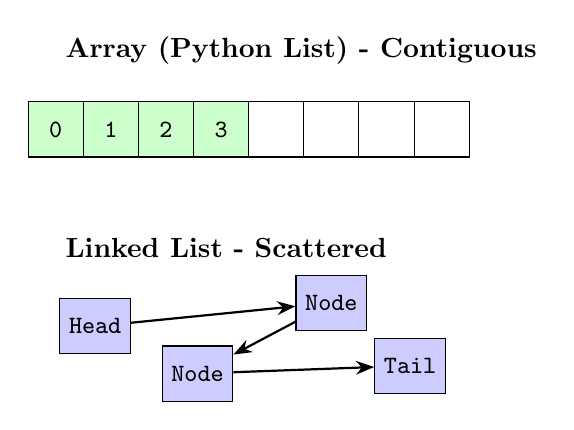
\begin{tikzpicture}[
    cell/.style={rectangle, draw, minimum size=0.7cm, font=\ttfamily\small},
    array/.style={fill=green!20},
    ll/.style={fill=blue!20}
]
    % Array memory
    \node[anchor=west] at (0, 1) {\textbf{Array (Python List) - Contiguous}};
    \foreach \i in {0,...,7} {
        \node[cell, \ifnum\i<4 array\fi] (a\i) at (\i*0.7, 0) {\ifnum\i<4 \i\fi};
    }

    % Linked List memory
    \node[anchor=west] at (0, -1.5) {\textbf{Linked List - Scattered}};
    \node[cell, ll] (l1) at (0.5, -2.5) {Head};
    \node[cell, ll] (l2) at (3.5, -2.2) {Node};
    \node[cell, ll] (l3) at (1.8, -3.1) {Node};
    \node[cell, ll] (l4) at (4.5, -3.0) {Tail};

    \draw[-{Stealth}, thick] (l1) -- (l2);
    \draw[-{Stealth}, thick] (l2) -- (l3);
    \draw[-{Stealth}, thick] (l3) -- (l4);

\end{tikzpicture}
\end{document}